%%% ---------------------------------------------------------------------------------
%%% Vorlage Abschlussarbeit (LaTeX)
%%% 
%%% V1   03/2017, Stefan Etschberger (HSA)
%%% V1.1 04/2021, rnw-hack für biblatex-run
%%% V2   05/2021, Titelblatt und Erweiterungen: Stefan Jansen (HSA)
%%% V2.1 05/2021, Trennung von R-Support und einfachem LaTeX: Phillip Heidegger (HSA)
%%% V2.2 01/2024, Anpassung an THA-Layout
%%% V3   01/2024, I18n
%%% V3.1 10/2024, Phillip Heideger, Online Version präferiert, Reparatur langes Inhaltsverzeichnis,
%%%               Erklärung Referenzen, blau für Refs & Links
%%% ---------------------------------------------------------------------------------
\documentclass[12pt,a4paper%
              ,oneside     % fuer PDF-Abgabe, bei Druck twoside
              ,titlepage
              ,DIV=13
              ,headinclude
              ,footinclude=false%
              ,cleardoublepage=empty%
              ,parskip=half,
              BCOR=0mm,
              ]{scrreprt}

\usepackage[utf8]{inputenc}
\usepackage[T1]{fontenc}

\usepackage[authorName={}
           ,authorEnrolmentNo={}
           ,authorStreet={}
           ,authorZip={}
           ,authorCity={}
           ,authorEMail={}
           ,authorPhone= {}
           ,authorSignaturePlace={}
           ,studyProgram={Mathematik}
           ,thesisType={Dokumentation}
           ,thesisTitle={NoSQL: Umsetzung der Semesteraufgabe mit Google Firestore}
           ,studyDegree=%
%                        {{Bachelor of Arts}}
%                        {{Bachelor of Engeneering}}
                        {{Bachelor of Science (B.\,Sc.)}}
%                        {{Master of Arts}}
%                        {{Master of Engeneering}}
%                        {{Master of Science (M.\,Sc.)}}
           ,faculty=% 
%                     {{Fakultät für \\ Angewandte \\ Geistes-  und  \\ Naturwissenschaften}}
%                     {{Fakultät für \\ Architektur und \\ Bauwesen}}
%                     {{Fakultät für \\ Elektrotechnik}}
%                     {{Fakultät für \\ Gestaltung}}
                      {{Fakultät für \\ Informatik}}
%                     {{Fakultät für \\ Maschinenbau und \\ Verfahrenstechnik}}, showDiesel=true
%                     {{Fakultät für \\ Wirtschaft}}
%           ,topicAssignment={\today}
%           ,submissionDate={\today}
%           ,defenseDate={\today}
%           ,nonDisclosure={false}
           ,supervisor={Prof.~Dr.~Frank N. Stein}
%           ,supervisorDeputy={Prof.~Dr.~Mario Huana}
%           ,language={en}
           ]{THA-docu}

% ====== mögliches Setup fürs PDFs =======
\hypersetup{
  colorlinks=true,
  allcolors = THAi-Blue, % oder THAred ??
  linktocpage  
}
% Siehe:
% https://ctan.net/macros/latex/contrib/hyperref/doc/hyperref-doc.pdf
% S. Kap. 5, S. 10 ff

% Ohne diese Zeile: Mit klickbaren links
% \hypersetup{draft}


% Literaturdatenbank (.bib-Datei) aus Citavi o.ä.
\bibliography{Literatur_docu}

\graphicspath{{Bilder/}}

\usepackage[font=small,labelfont=bf]{caption}
\DeclareCaptionLabelFormat{something}{#2.#1.}
\captionsetup[lstlisting]{labelformat=something}

\usepackage{chngcntr}
\usepackage{float}

\counterwithout{figure}{chapter}
\begin{document}

% Sprachauswahl zum Umschalten innerhalb des Textes. 
% Alternativen: \thesisLanguage, ngerman, english
\selectlanguage{\thesisLanguage}

\pagenumbering{roman}
\setcounter{page}{1}

\THAtitlepage

\tableofcontents

%%% --------------------------------------------------
%%% Ab hier: Inhalt
%%% --------------------------------------------------

\setcounter{page}{1}
\pagenumbering{arabic}

\chapter{Ausgangssituation}
\label{einleitung}

In unserer neuen Position im Datenbank-Team haben wir von unserem Vorgänger eine relationale Kurs-Datenbank übernommen. Laut Vorgabe des Managements soll diese nun in eine moderne NoSQL-Datenbank überführt werden.

Da keine strukturierte Übergabe stattfand, stand uns lediglich ein SQL-Dump der alten Datenbank zur Verfügung. Um die Datenstruktur besser zu verstehen und einen Überblick über die enthaltenen Tabellen und deren Beziehungen zu gewinnen, haben wir diesen Dump zunächst in ein Entity-Relationship-Diagramm (ERD) überführt.

Abbildung~\ref{fig:enr-old} zeigt das daraus entstandene ER-Diagramm, das insgesamt neun relationale Tabellen umfasst:

\begin{figure}[htbp]
	\centering
	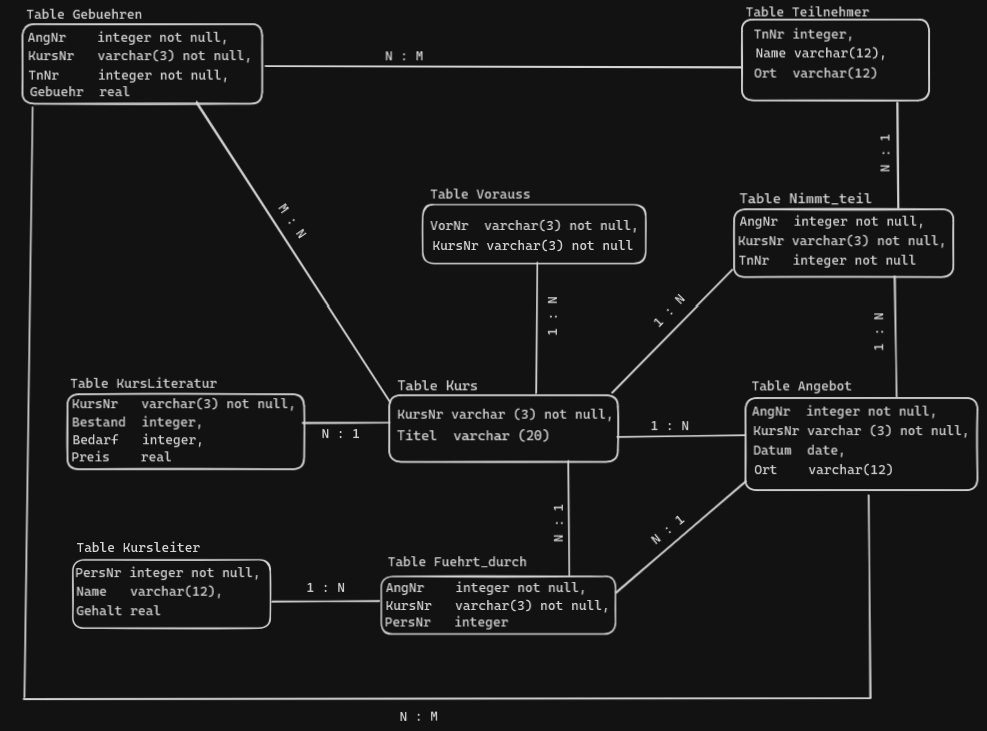
\includegraphics[width=\dimexpr0.7\linewidth]{img/SQL_DUMP_ERM.png}
	\caption{Entity-Relationship-Diagramm der ursprünglichen relationalen Struktur}
	\label{fig:enr-old}
\end{figure}

Auf Basis dieser Analyse entschieden wir uns, die Struktur in eine dokumentenbasierte NoSQL-Datenbank zu übertragen. Dabei war es uns wichtig, die ursprüngliche logische Struktur möglichst beizubehalten, sie jedoch gleichzeitig so zu modellieren, dass sie den Prinzipien und Stärken eines dokumentenorientierten Datenmodells entspricht.

\chapter{Entscheidung für eine NoSQL-Datenbank}

Zur Auswahl einer geeigneten NoSQL-Datenbank haben wir zunächst das \textit{DB-Engines Ranking} (\url{https://db-engines.com/en/ranking}) als Orientierungshilfe herangezogen. Dieses Ranking bietet eine fundierte Übersicht über die aktuell am weitesten verbreiteten Datenbanktechnologien.

Nach einer kurzen Recherche hinsichtlich Verbreitung, Dokumentation und Community-Support fiel unsere Wahl auf \textbf{Google Cloud Firestore}. Ausschlaggebend war neben den technischen Eigenschaften und der guten Integration in das Node.js-Ökosystem auch unser persönliches Interesse an der Arbeit mit Firebase-Technologien.

\section{Google Cloud Firestore}

Google Cloud Firestore ist eine dokumentenbasierte NoSQL-Datenbank, in der Daten in sogenannten \textit{Collections} organisiert sind. Jede Collection kann beliebig viele \textit{Dokumente} enthalten, die wiederum hierarchisch strukturierte \textit{Subcollections} besitzen können. 

Die einzelnen Dokumente bestehen aus Feldern in Form von Schlüssel-Wert-Paaren und ähneln in ihrer Struktur stark JSON-Objekten. Dieses flexible Datenmodell ermöglicht die effiziente Speicherung von semistrukturierten Informationen.

Zu den zentralen Merkmalen von Firestore gehören die Unterstützung verschachtelter Datenstrukturen, Arrays, Referenzen auf andere Dokumente sowie spezielle Datentypen wie Zeitstempel. Dadurch lassen sich auch komplexe, objektähnliche Datenmodelle direkt und modellnah abbilden \cite{Kesavan.2023, Firebase.2025, FirebaseDatenmodell.2025}.

Die konkrete Umsetzung dieser Struktur in unserem Projekt wird in Kapitel~\ref{struktur-chapter} ausführlich dargestellt.

\section{Abfragesprache von Firestore}
\label{sprache-firestore}

Die Standardabfragesprache von Google Cloud Firestore ist keine deklarative Sprache wie SQL, sondern eine methodenbasierte API, die über verschiedene Programmiersprachen hinweg verfügbar ist. Firestore stellt hierfür offizielle SDKs bereit, unter anderem für JavaScript, TypeScript, Python, Java und Kotlin \cite{GoogleCloudQueries.2025}.

Die Interaktion mit der Datenbank erfolgt über eine Befehlskette aus Methodenaufrufen, mit denen sich Daten lesen, filtern, sortieren und paginieren lassen. Dabei orientieren sich die Methoden am zugrunde liegenden dokumentenbasierten Modell und bieten eine intuitive Möglichkeit, auf Daten zuzugreifen.

Abbildung~\ref{fig:code-example-0} zeigt ein einfaches Beispiel für eine Abfrage in Firestore mit JavaScript. Hier wird nach allen Städten gesucht, bei denen das Feld \texttt{capital} auf \texttt{true} gesetzt ist, sortiert nach der Bevölkerungszahl:

\begin{figure}[H]
	\centering
	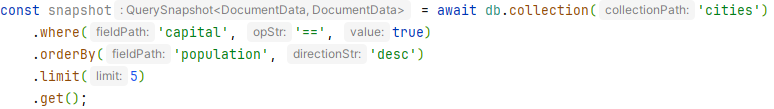
\includegraphics[width=\linewidth]{img/code_example_0.png}
	\caption{Beispiel einer Abfrage in Firestore}
	\label{fig:code-example-0}
\end{figure}

Im Gegensatz zu SQL müssen bei dieser Art von Abfragen Joins, Aggregationen und komplexere Operationen vom Client übernommen werden. Das bedeutet, dass manche Auswertungen – wie etwa das Zusammenführen mehrerer Datensätze – durch zusätzliche Logik im Anwendungscode umgesetzt werden müssen.

In unserem Projekt haben wir uns bewusst für die Verwendung von \textbf{TypeScript} entschieden, um die Stärken der Firestore-API mit statischer Typprüfung zu kombinieren. Dies war insbesondere im Hinblick auf die Datenmigration aus der relationalen Struktur von Vorteil, da wir so die ursprünglichen Datentypen in Form von Interfaces abbilden und validieren konnten.

Wie genau wir mithilfe von TypeScript und sogenannten \textit{Convertern} eine durchgehende Typsicherheit im Zugriff auf Firestore erreicht haben, wird ausführlich in Kapitel~\ref{typ-sicherheit-chapter} erläutert.

\section{Lokale Nutzung}

Da Google Cloud Firestore eine cloudbasierte Datenbank ist, standen wir vor der Herausforderung, sie lokal zu betreiben – denn die Nutzung einer Cloud-Lösung war in unserem Fall nicht zulässig. Für diesen Zweck stellt Firebase die sogenannte \textit{Local Emulator Suite} zur Verfügung. Dabei handelt es sich um eine Sammlung von Dienstemulatoren, die das Verhalten der echten Firebase-Dienste lokal nachbilden \cite{EmulatorSuite.2025}.

Für unser Projekt reichte der Einsatz des Firestore-Emulators sowie der zugehörigen Benutzeroberfläche aus. Die Einrichtung erfolgte lokal durch die Installation von \textit{Node.js}, dem \textit{Java JDK} sowie der \textit{Firebase CLI}. Mit wenigen Konfigurationsbefehlen ließ sich anschließend die erforderliche Datei \texttt{firebase.json} generieren. Dieses Setup entspricht dem von Firebase empfohlenen Vorgehen für die lokale Entwicklung \cite{EmulatorInsall.2025}.

Abbildung~\ref{fig:emulator-ui} zeigt einen Ausschnitt aus der Benutzeroberfläche des Emulators:

\begin{figure}[H]
	\centering
	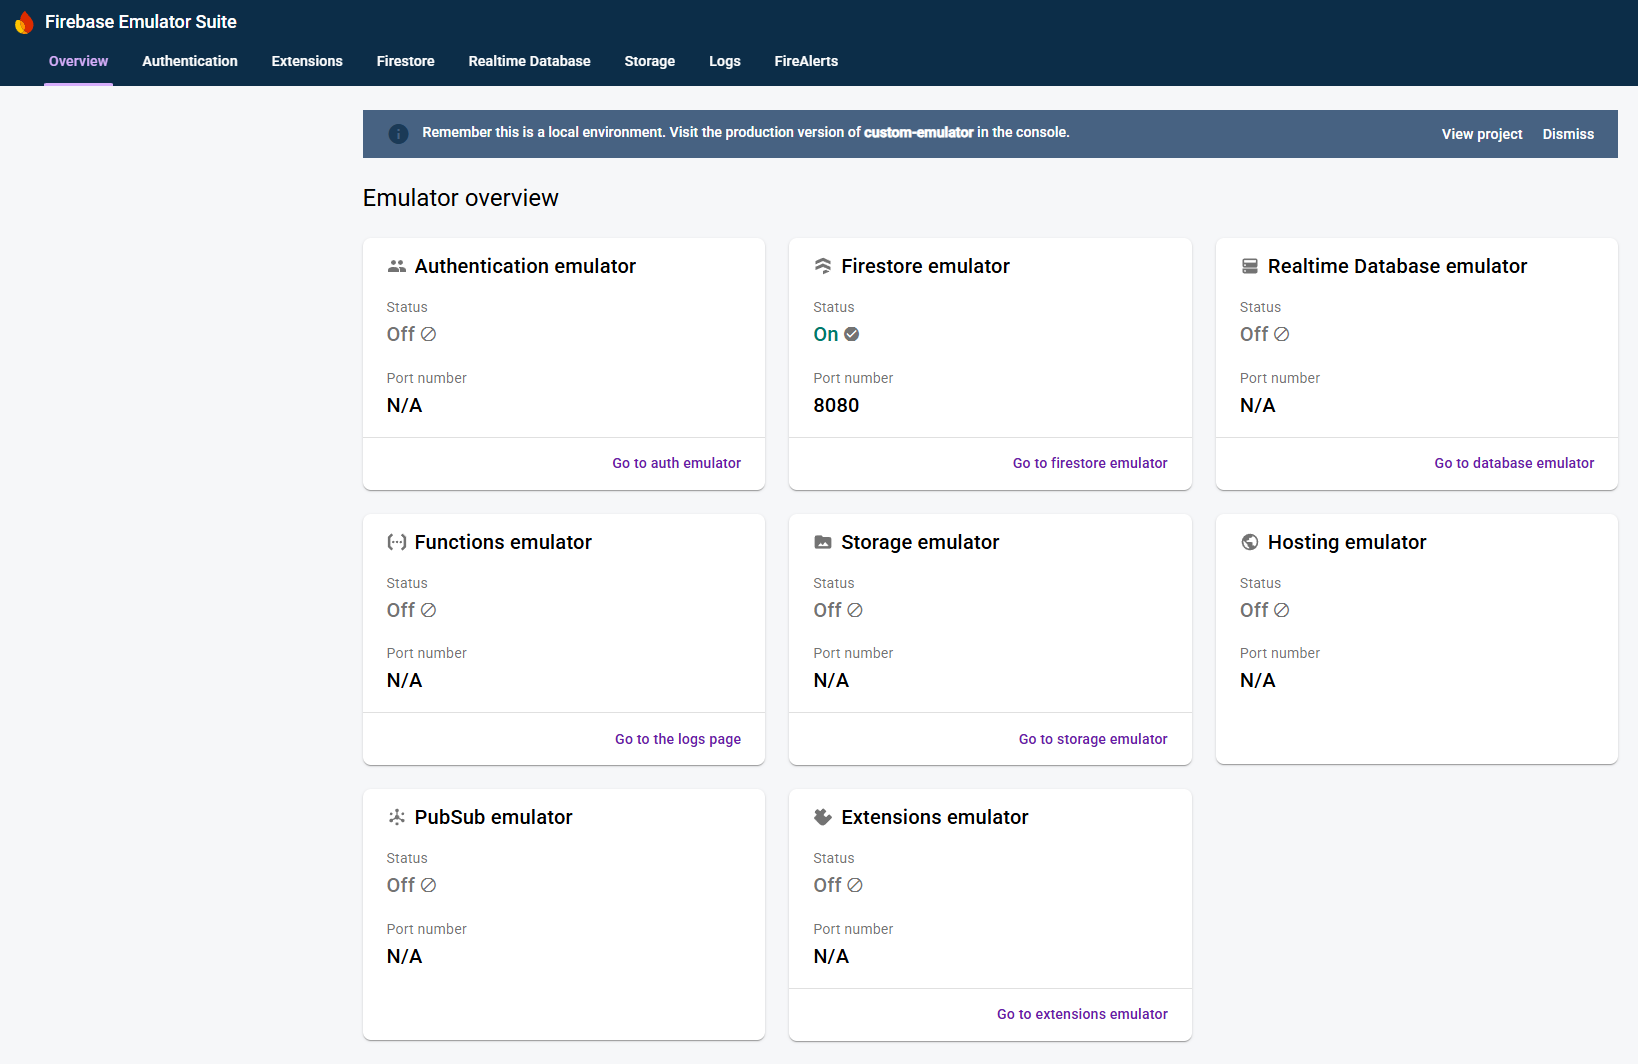
\includegraphics[width=\linewidth]{img/emulator_ui.png}
	\caption{Auszug aus der UI der Local Emulator Suite}
	\label{fig:emulator-ui}
\end{figure}

\subsection{Versuchter alternativer Ansatz zur lokalen Nutzung}

Neben der empfohlenen lokalen Installation der Emulator Suite haben wir auch versucht, die Firestore-Emulatorumgebung mithilfe von Docker bereitzustellen. Ziel war es, die notwendigen Tools nicht direkt auf unseren eigenen Systemen installieren zu müssen.

Dazu haben wir verschiedene Beiträge, Artikel und GitHub-Repositories recherchiert und unterschiedliche Ansätze ausprobiert, unter anderem:

\begin{enumerate}
	\item \url{https://github.com/PathMotion/firestore-emulator-docker}
	\item \url{https://hub.docker.com/r/mtlynch/firestore-emulator/}
	\item \url{https://medium.com/@jens.skott_65388/simplifying-firebase-emulation-with-docker-a-guide-to-local-development-and-testing-0c3c33fd92c7}
	\item \url{https://github.com/ridedott/firestore-emulator-docker/blob/master/Dockerfile}
\end{enumerate}

Zwar ließ sich die Emulator Suite grundsätzlich innerhalb eines Docker-Containers starten und auch die Benutzeroberfläche aufrufen, jedoch traten in der praktischen Nutzung erhebliche Einschränkungen auf. Das Hauptproblem bestand darin, dass der Zugriff auf die Datenbank aus externen Skripten heraus nicht zuverlässig funktionierte – insbesondere die Weiterleitung der Ports (Expose) verursachte Schwierigkeiten.

Eine alternative Lösung wäre gewesen, sämtliche Skripte direkt innerhalb des Containers auszuführen. Dieses Vorgehen erschien uns jedoch in Bezug auf Wartbarkeit und Entwicklungsfluss zu umständlich. Aufgrund dieser Einschränkungen haben wir uns letztlich für den von Firebase vorgesehenen Weg mit lokaler Installation entschieden, der sich als unkompliziert und stabil erwiesen hat.

\chapter{Aufbau der Datenstruktur}
\label{struktur-chapter}

Für die Überführung der in Kapitel~\ref{einleitung} beschriebenen relationalen Struktur haben wir die Vorteile eines dokumentenbasierten Datenmodells – wie es Google Firestore bietet – gezielt genutzt. Die finale Datenstruktur ist dabei nicht von Anfang an in ihrer jetzigen Form entstanden, sondern wurde im Laufe der Projektarbeit mehrfach überarbeitet und optimiert. Ziel war es, eine Lösung zu entwickeln, die sowohl den ursprünglichen Datenbeziehungen gerecht wird als auch eine effiziente Umsetzung der geforderten Abfragen ermöglicht.

Die resultierende Struktur ist in Abbildung~\ref{fig:structure} visualisiert:

\begin{figure}[H]
	\centering
	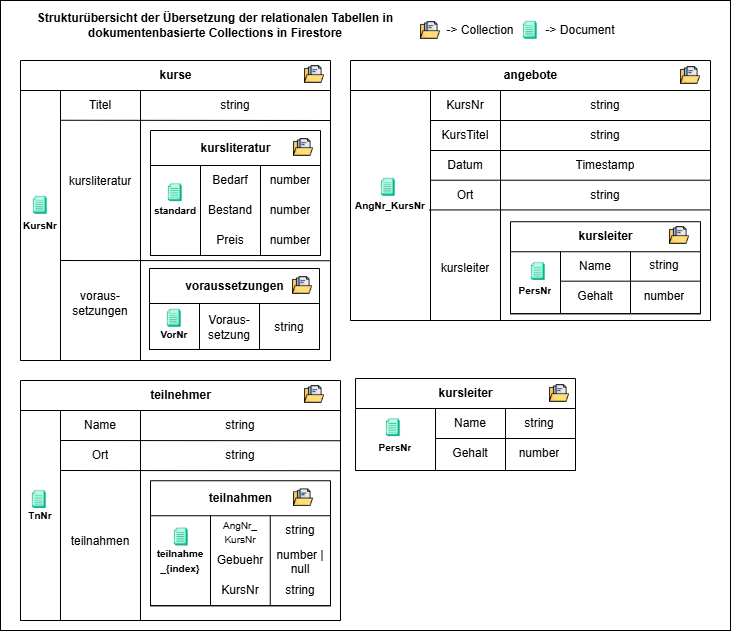
\includegraphics[width=\dimexpr0.9\linewidth]{img/StrukturFirestore.png}
	\caption{Struktur der Daten in Firestore}
	\label{fig:structure}
\end{figure}

Aus den insgesamt neun relationalen Tabellen wurden vier Haupt-Collections abgeleitet: \texttt{kurse}, \texttt{angebote}, \texttt{teilnehmer} und \texttt{kursleiter}. Dabei wurden einige ursprünglich eigenständige Tabellen als Sub-Collections integriert:

\begin{itemize}
	\item In \texttt{kurse} befinden sich die Sub-Collections \texttt{kursliteratur} (ursprünglich: \texttt{KursLiteratur}) und \texttt{voraussetzungen} (ursprünglich: \texttt{Vorauss}).
	\item In \texttt{teilnehmer} ist die Sub-Collection \texttt{teilnahmen} untergebracht (ursprünglich: \texttt{Nimmt\_teil}), wobei die ehemals separate Tabelle \texttt{Gebuehren} nun als Feld innerhalb der Teilnahme gespeichert ist.
	\item Die Collection \texttt{kursleiter} entspricht nahezu direkt der alten Tabelle gleichen Namens.
	\item Die Collection \texttt{angebote} wurde am stärksten angepasst: Neben der Sub-Collection \texttt{kursleiter}, in der relevante Kursleiterdaten (redundant) gespeichert sind, wird dort zusätzlich der \texttt{KursTitel} direkt im Angebot abgelegt.
\end{itemize}

Die redundante Speicherung des Kurstitels sowie der Kursleiterdaten wurde bewusst gewählt. In Firestore sind komplexe JOINs, wie sie in relationalen Datenbanken üblich sind, nicht möglich. Um performante Abfragen zu ermöglichen und unnötige Mehrfachabfragen zu vermeiden, ist dieses Vorgehen sogar empfohlen und gilt als \textit{Best Practice} im Umgang mit NoSQL-Datenbanken \cite{Estuary.2025}.

Insgesamt entspricht die von uns gewählte Struktur dem Paradigma einer dokumentenorientierten Datenbank. Sie erwies sich im Verlauf der Umsetzung als robust und praxistauglich, insbesondere im Hinblick auf die Bearbeitung der gestellten Aufgaben. Gleichzeitig bringt die Entscheidung für redundante Datenhaltung gewisse Herausforderungen mit sich – insbesondere bei \texttt{update}- und \texttt{delete}-Operationen. Diese Aspekte werden in den Kapiteln~\ref{update-label} und \ref{delete-label} näher erläutert.

\chapter{Typsicherheit und Abfragen mit TypeScript}
\label{typ-sicherheit-chapter}

Wie bereits in Kapitel~\ref{sprache-firestore} erwähnt, haben wir uns bei der Implementierung für TypeScript als Abfragesprache entschieden. Der Hauptgrund dafür war, dass Firestore standardmäßig keine Typsicherheit bietet. Das Datenbanksystem selbst ist schemalos, sodass die Validierung von Datentypen vollständig in der Anwendungsschicht erfolgen muss.

Da wir möglichst nah an den Datentypen der ursprünglichen relationalen Struktur bleiben wollten, haben wir in TypeScript entsprechende Interfaces für alle Tabellen definiert. Für die Datenbankkommunikation kam das offizielle npm-Paket \texttt{@google-cloud/firestore} (\url{https://www.npmjs.com/package/@google-cloud/firestore}) zum Einsatz, das wir mit unseren Typdefinitionen kombiniert haben, um eine durchgängige Typsicherheit zu gewährleisten.

Abbildung~\ref{fig:types} zeigt einen Auszug unserer zentralen Typdefinitionen:

\begin{figure}[H]
	\centering
	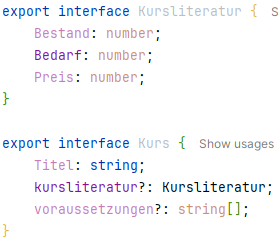
\includegraphics{img/types.png}
	\caption{Auszug aus unseren Typdefinitionen}
	\label{fig:types}
\end{figure}

Damit diese Typen nicht nur in unserem Anwendungscode verwendet werden, sondern auch beim Zugriff auf die Firestore-Datenbank wirksam sind, haben wir zusätzlich sogenannte \textit{Converter} implementiert. Diese ermöglichen es, typisierte Daten aus der Datenbank zu lesen und wieder zurückzuschreiben – und zwar im Einklang mit den definierten TypeScript-Interfaces.

\begin{figure}[H]
	\centering
	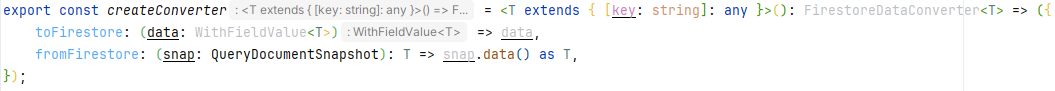
\includegraphics[width=\linewidth]{img/converter.png}
	\caption{Definition unserer Converter}
	\label{fig:converter}
\end{figure}

Wie in Abbildung~\ref{fig:converter} zu sehen, implementiert unser Converter-Objekt zwei zentrale Methoden: \texttt{fromFirestore} konvertiert das rohe Datenobjekt aus Firestore in einen konkreten TypeScript-Typ, während \texttt{toFirestore} dafür sorgt, dass nur strukturkonforme Objekte in die Datenbank geschrieben werden. 

Im Zusammenspiel mit der Methode \texttt{.withConverter()} des Firestore-SDK konnten wir so eine durchgängige Typprüfung bei allen Lese- und Schreibvorgängen realisieren. Abbildung~\ref{fig:converter_example} zeigt ein Beispiel für den praktischen Einsatz des Converters im Code:

\begin{figure}[H]
	\centering
	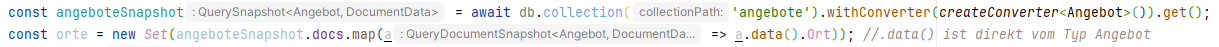
\includegraphics[width=\linewidth]{img/converter_example.png}
	\caption{Beispiel für die Verwendung eines Converters}
	\label{fig:converter_example}
\end{figure}

\paragraph{\textbf{Praktische Vorteile.}} Der Einsatz dieser Technik brachte mehrere Vorteile mit sich:

\begin{itemize}
	\item \textbf{Reduktion von Fehlern:} Typfehler, vergessene Felder oder falsche Datentypen wurden bereits zur Entwicklungszeit durch den TypeScript-Compiler erkannt.
	\item \textbf{Bessere Wartbarkeit:} Änderungen an Datenstrukturen waren dank der zentralen Typdefinitionen leicht nachvollziehbar und systemweit konsistent anpassbar.
	\item \textbf{Konsistenz in beiden Richtungen:} Die gleiche Datenstruktur wurde sowohl beim Einlesen als auch beim Schreiben verwendet – ohne doppelte Validierung oder manuelle Typzuweisungen.
\end{itemize}

\paragraph{\textbf{Abgrenzung zum Firestore-Modell.}} Firestore selbst stellt – anders als relationale Datenbanken – kein festes Schema zur Verfügung. Durch die Kombination aus TypeScript und Convertern konnten wir dieses Defizit vollständig auf Anwendungsebene kompensieren. Besonders im Rahmen der Migration einer bestehenden SQL-Datenbank erwies sich dieser Ansatz als äußerst hilfreich.

\section{Initiales Laden der Daten nach Firestore}

Nachdem die Datenstruktur definiert und die Nutzung von TypeScript-Typen sowie Convertern zur Gewährleistung der Typsicherheit erläutert wurde, bestand der nächste Schritt darin, die Ausgangsdaten in die Firestore-Datenbank zu überführen. Dies war notwendig, um anschließend alle \textit{read}-, \textit{update}- und \textit{delete}-Operationen ausführen zu können.

Die bereitgestellten Daten wurden zunächst in mehreren \texttt{.json}-Dateien organisiert. Mithilfe eines eigens entwickelten \textit{Load-Skripts} konnten diese anschließend automatisiert in Firestore importiert werden. Dabei war es entscheidend, dass für jede Datei der passende \texttt{Converter} in Kombination mit den zuvor definierten TypeScript-Typen verwendet wurde.

Besonderes Augenmerk lag auf der korrekten Behandlung von Sub-Collections, da diese – anders als in relationalen Datenbanken – nicht automatisch mit dem Hauptdokument gespeichert werden, sondern explizit separat geschrieben werden müssen.

Obwohl dieser Initialimport technisch gesehen relativ einfach umzusetzen war, musste er sehr sorgfältig durchgeführt werden, um sicherzustellen, dass sämtliche Daten im richtigen Format und an der korrekten Stelle gespeichert werden. Nur so konnten wir garantieren, dass alle nachfolgenden Abfragen erwartungsgemäß funktionieren.

%ab hier im moment nur KI generiert
\chapter{Herausforderungen bei den Read-Abfragen}

% @Leonelle habe dein Text einfach mit KI nochmal bisschen überarbeiten lassen, wenn es dir nicht gefällt, können wir es gerne rückgängig machen
Bei der Umsetzung der Leseabfragen in Firestore traten mehrere Einschränkungen zutage, die im Vergleich zu klassischen relationalen Datenbanken zusätzliche Komplexität mit sich brachten. Im Folgenden sind zwei zentrale Punkte exemplarisch erläutert:

\begin{enumerate}
	\item \textbf{Keine Unterstützung für JOINs:} 
	In SQL können Daten aus mehreren Tabellen mithilfe von \texttt{JOIN}-Operationen direkt miteinander verknüpft werden. In Firestore existiert eine solche Funktionalität nicht. Um beispielsweise die Informationen zu einem Angebot gemeinsam mit dem zugehörigen Kurstitel zu laden (wie in Abfrage \textbf{d}), mussten zunächst alle Dokumente aus der Collection \texttt{angebote} gelesen und anschließend für jedes einzelne Dokument das passende Kursdokument aus der Collection \texttt{kurse} manuell nachgeladen werden. Dies führt bei größeren Datenmengen zu einem erheblichen Mehraufwand und einer höheren Anzahl an Leseoperationen – was sich negativ auf die Performance und potenziell auf die Kosten auswirken kann.
	\item \textbf{Eingeschränkte Aggregatfunktionen:}
    Firestore unterstützt inzwischen einfache Aggregationen wie \texttt{count()}, allerdings nur für die Gesamtanzahl von Dokumenten, die bestimmte Kriterien erfüllen. Komplexe Aggregationen wie \texttt{GROUP BY} oder \texttt{HAVING COUNT(*)}, wie sie in SQL üblich sind, sind in Firestore weiterhin nicht möglich. In Abfrage \textbf{i} (Kurse mit mindestens zwei Teilnehmern) musste daher in Firestore ein eigenes Zählerobjekt im Anwendungscode erstellt werden, das sämtliche Teilnahme-Dokumente durchläuft und die Anzahl pro Kursangebot manuell berechnet. Das verlagert die Logik vollständig in die Anwendungsebene und erhöht damit den Entwicklungsaufwand.
	% \item \textbf{Keine Aggregatfunktionen wie \texttt{COUNT}, \texttt{AVG} oder \texttt{GROUP BY}:} 
	% Firestore bietet keine eingebauten Funktionen zur Aggregation von Daten. Eine typische SQL-Abfrage wie „Gib alle Kurse mit mindestens zwei Teilnehmern aus“ (siehe Abfrage \textbf{i}) müsste in SQL lediglich eine Zeile mit \texttt{GROUP BY} und \texttt{HAVING COUNT(*) >= 2} umfassen. In Firestore hingegen musste ein eigenes Zählerobjekt im Anwendungscode erstellt werden, das sämtliche Teilnahme-Dokumente durchläuft und die Anzahl pro Kursangebot manuell berechnet. Das verlagert die Logik vollständig in die Anwendungsebene und erhöht damit den Entwicklungsaufwand.
\end{enumerate}

% @Gregor hier kannst du gerne noch mehr Sachen einfügen und ausführlicher etc. vlt auch mit Quellen oder iwas noch
Darüber hinaus ist der direkte Zugriff auf Sub-Collections ebenfalls nicht ohne Weiteres möglich – etwa, wenn man aus einer übergeordneten Collection alle enthaltenen Sub-Dokumente aggregiert betrachten möchte. Auch hierfür sind zusätzliche Leseoperationen und individuelle Nachladeprozesse erforderlich.

Diese Einschränkungen zeigen exemplarisch, dass NoSQL-Systeme wie Firestore zwar flexibel in der Datenmodellierung sind, jedoch bei komplexeren Auswertungen oft zusätzliche clientseitige Logik erforderlich machen.

\chapter{Herausforderungen bei den Update-Abfragen}
\label{update-label}

% @Peter, dass hier ist obv nicht richtig und nur für die Theorie generiert, pass das bitte auf unser Projekt mit Quellen von offizieler Firebase Doku z.B. zu batch writes und transaktionen
Ein wesentliches Merkmal dokumentenbasierter NoSQL-Datenbanken wie Firestore ist die bewusste Entscheidung für Redundanz, um Abfragen zu beschleunigen und komplexe JOINs zu vermeiden. Diese Modellierungsfreiheit bringt jedoch Herausforderungen mit sich – insbesondere bei \texttt{update}-Operationen.

Ein konkretes Beispiel in unserem Projekt ist der redundante \texttt{KursTitel}, der sowohl in der Collection \texttt{kurse} als auch mehrfach in der Collection \texttt{angebote} gespeichert wird. Wird der Titel eines Kurses geändert, muss sichergestellt werden, dass alle zugehörigen Angebote ebenfalls aktualisiert werden, um Inkonsistenzen zu vermeiden.

In relationalen Datenbanken würde dies durch eine zentrale Normalisierung und Fremdschlüsselbeziehungen automatisch sichergestellt werden. In Firestore hingegen ist die Konsistenz zwischen redundanten Feldern Aufgabe der Anwendung.

Zur Lösung dieses Problems bietet Firestore sogenannte \textit{Batch Writes} und \textit{Transaktionen} an. Bei einem Batch Write können mehrere Dokumente in einem einzigen atomaren Schritt aktualisiert werden. Transaktionen ermöglichen zusätzlich, innerhalb eines Konsistenzkontextes zu lesen und zu schreiben – was insbesondere dann hilfreich ist, wenn Bedingungen geprüft werden müssen, bevor geschrieben wird.

In unserem Projekt war der Einsatz von \texttt{Batch Writes} die bevorzugte Methode, da wir genau wussten, welche Felder aktualisiert werden müssen und keine Abhängigkeiten zwischen den Lese- und Schreibvorgängen bestanden. Änderungen am Kurstitel konnten so gezielt auf alle betroffenen \texttt{angebote}-Dokumente angewendet werden.

Trotzdem bleibt zu beachten, dass Firestore keine automatische Änderungsweitergabe (wie \texttt{ON UPDATE CASCADE} in SQL) unterstützt. Entwickler:innen müssen sich dieser Limitierung bewusst sein und gegebenenfalls eigene Routinen oder Skripte entwickeln, um die Konsistenz sicherzustellen.

\chapter{Herausforderungen bei den Delete-Abfragen}
\label{delete-label}

% @Jana das ist obv noch komplett falsch hier, geht aber um die Theorie etc, pass das bitte an auf unser Projekt und vlt ist was sinnvolles dabei + maybe Quellen?
Neben der Aktualisierung redundanter Daten stellt auch das Löschen von Dokumenten in Firestore eine besondere Herausforderung dar – insbesondere dann, wenn Daten mehrfach gespeichert oder in Sub-Collections organisiert sind.

Ein typisches Beispiel ist das Löschen eines Kurses: Während in einer relationalen Datenbank mit referenzieller Integrität und \texttt{ON DELETE CASCADE} automatisch alle abhängigen Einträge (z.\,B. Angebote oder Teilnahmen) entfernt werden können, existiert eine solche automatische Löschkaskade in Firestore nicht.

Wird ein Dokument in einer Haupt-Collection gelöscht (z.\,B. ein Kurs), so bleiben zugehörige Dokumente in Sub-Collections oder redundanten Kopien (etwa in \texttt{angebote.kursleiter}) bestehen – es sei denn, sie werden explizit mitgelöscht. Das kann zu Inkonsistenzen und veralteten Daten führen, wenn keine zusätzliche Logik zur Datenpflege implementiert wird.

Zur Umsetzung konsistenter Löschvorgänge haben wir daher ein eigenes Skript verwendet, das beim Entfernen eines Hauptdokuments auch alle zugehörigen Sub-Dokumente und Kopien löscht. Firestore bietet hierfür keine eingebaute Funktion, aber durch den Einsatz von sogenannten \texttt{batch}– oder \texttt{recursive delete}-Operationen in Kombination mit manueller Traversierung der Dokumentstruktur lässt sich diese Funktionalität nachbilden.

Alternativ könnte man auch auf serverseitige Mechanismen wie \textit{Firebase Cloud Functions} zurückgreifen, die automatisch auf Datenänderungen reagieren können. Diese Lösung war in unserem Projekt jedoch nicht erlaubt, da wir ausschließlich lokal mit der Emulator Suite arbeiten durften und auf Cloud-Integrationen verzichten mussten.

Somit liegt die Verantwortung für konsistentes Löschen bei der Anwendungsschicht – ein bedeutender Unterschied zu relationalen Systemen, der insbesondere bei komplexeren Datenmodellen berücksichtigt werden muss.

\chapter{Fazit}

Die Migration einer relationalen Kursdatenbank in eine dokumentenbasierte NoSQL-Datenbank wie Google Cloud Firestore stellte sich als ebenso herausfordernd wie lehrreich heraus. Während relationale Datenbanken durch ihr starres Schema und eingebaute Beziehungen wie \texttt{JOINs}, \texttt{GROUP BY} oder referenzielle Integrität eine hohe Datenkonsistenz und Abfrageflexibilität bieten, verlangt das Arbeiten mit Firestore ein grundsätzlich anderes Denken: Daten müssen häufiger redundant gespeichert, Abfragen logisch vereinfacht und viele Operationen in die Anwendungsschicht verlagert werden.

Durch die Verwendung von TypeScript und Convertern konnten wir diesem schemalosen Ansatz eine starke Typsicherheit entgegensetzen und so sowohl bei der Datenmodellierung als auch bei der Datenverarbeitung präzise und konsistente Strukturen gewährleisten. Besonders hilfreich war dieser Ansatz im Kontext der ursprünglichen relationalen Struktur, da wir so viele der alten Konzepte typisiert beibehalten konnten.

Die Herausforderungen im Bereich der Lese-, Update- und Delete-Operationen haben deutlich gemacht, dass NoSQL-Systeme zwar hohe Flexibilität bieten, dafür aber auf Kosten automatischer Konsistenzmechanismen. Durch manuelle Scripte, gezielte Datenmodellierung und die Nutzung von Batch-Operationen konnten wir dennoch eine robuste und nachvollziehbare Lösung implementieren.

Die Entscheidung für Firestore hat sich trotz der technischen Einschränkungen insgesamt als sinnvoll erwiesen – vor allem aufgrund der leichten Einstiegsmöglichkeiten, der guten lokalen Entwicklungsumgebung (Emulator Suite) sowie der vollständigen Kontrolle über Datenstruktur und Zugriff.

Abschließend lässt sich sagen, dass dokumentenbasierte Datenbanken wie Firestore ideal für Projekte mit semistrukturierten Daten und klar definierten Zugriffsmustern geeignet sind. Gleichzeitig ist es entscheidend, sich der Einschränkungen bewusst zu sein – insbesondere im Hinblick auf relationale Operationen, Aggregationen und automatische Konsistenz.

Das Projekt hat nicht nur unsere Kenntnisse in Firestore, TypeScript und NoSQL-Datenmodellierung vertieft, sondern auch ein praktisches Verständnis dafür geschaffen, wie sich klassische relationale Datenbankmodelle in moderne, flexible Cloudsysteme überführen lassen.


\appendix

% Selbständigkeitserklärung
%\AuthorDeclaration


%\listoffigures % Abbildungsverzeichnis
%\listoftables % Tabellenverzeichnis

% --------------------------------------------------
% Bibliographie
% --------------------------------------------------
\renewcommand{\bibfont}{\footnotesize}
\printbibliography[title={Literaturverzeichnis}, 
                   heading=bibintoc]


% --------------------------------------------------
% Index
% --------------------------------------------------
{\setkomafont{section}{\Huge} % temporarily set chapter font
\printindex
}

\end{document}
